In the following part of this report, the color detection will be used to distinguish color light points projected by a luminous source on a Martian rocks from its background. In order to implement this color detection, the HSV color model needs to be defined, as well as some morphological operations. 

\subsection{HSV Color System}
HSV stands for Hue Saturation Value. It is a color system which allows the separation of the color components from the intensity, unlike RGB system. It is more intuitive to find a plain object by varying HSV parameters.

The Hue designates the color itself. As it can be seen on the figure \ref{fig:HSV}, the color is determined by an angle between 0\degree and 360\degree. Red corresponds to 0�, green to 120� and blue to 240�. OpenCV range is 0-180. Changing the Saturation will affect the intensity of the color. A low value indicates a dull color. The Value has an impact on the luminosity of the color. Decreasing this value makes the color darker. The S and V are varying between 0 and 1 but the OpenCV range is 0-255.

\begin{figure}[H]
  \centering
  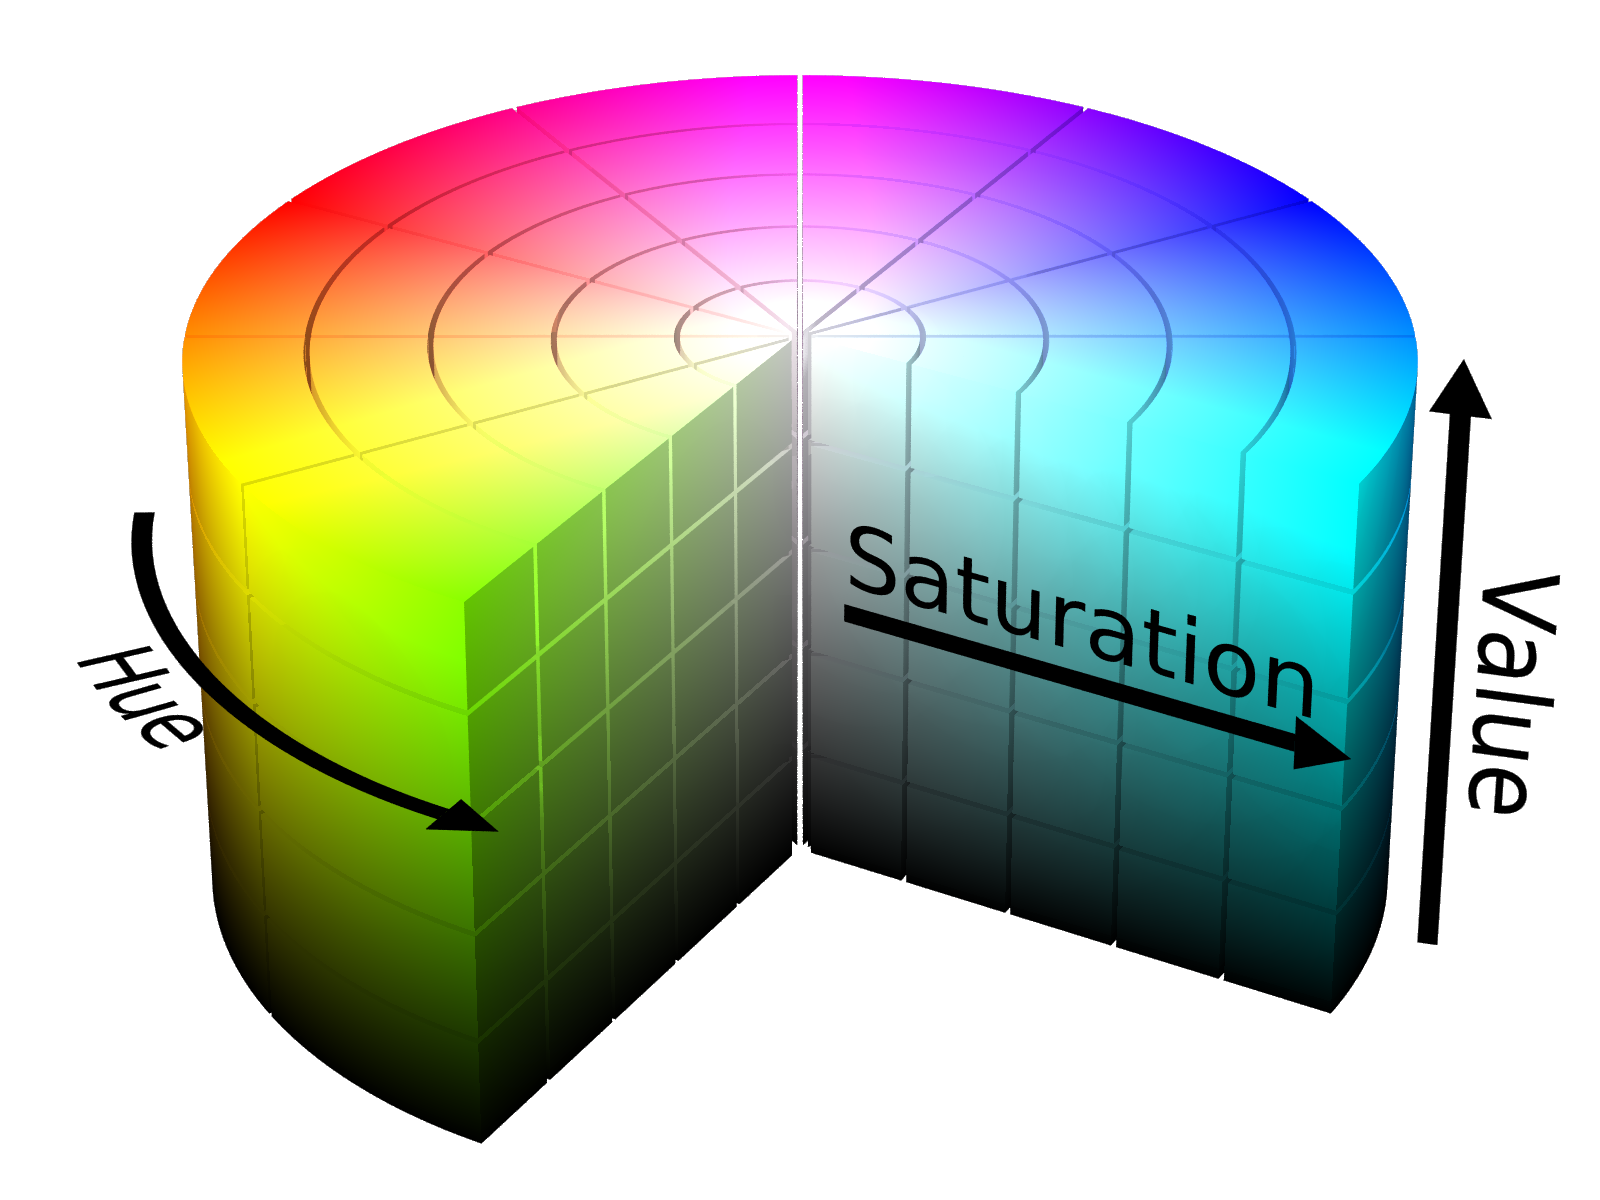
\includegraphics[scale=0.15]{fig/HSV.png}
  \caption{HSV diagram \cite{wiki:hsv}}
  \label{fig:HSV}
\end{figure}

\subsection{Morphological Operations \cite{bradski2008learning}}
The morphological operations on a binary image consists in applying a structuring element to each pixel of the object parts to reshape them. Two basic operations will be used later on and are explained here: the erosion and the dilation. Detailed diagram of the erosion and dilation can be found below (figures \ref{fig:erosion} and \ref{fig:dilation}). It should be noticed that for more legibility, the background is in white and the object in color. It will however be assumed that the pixels of the object have a value superior to the background.

\begin{figure}[h]
  \centering
  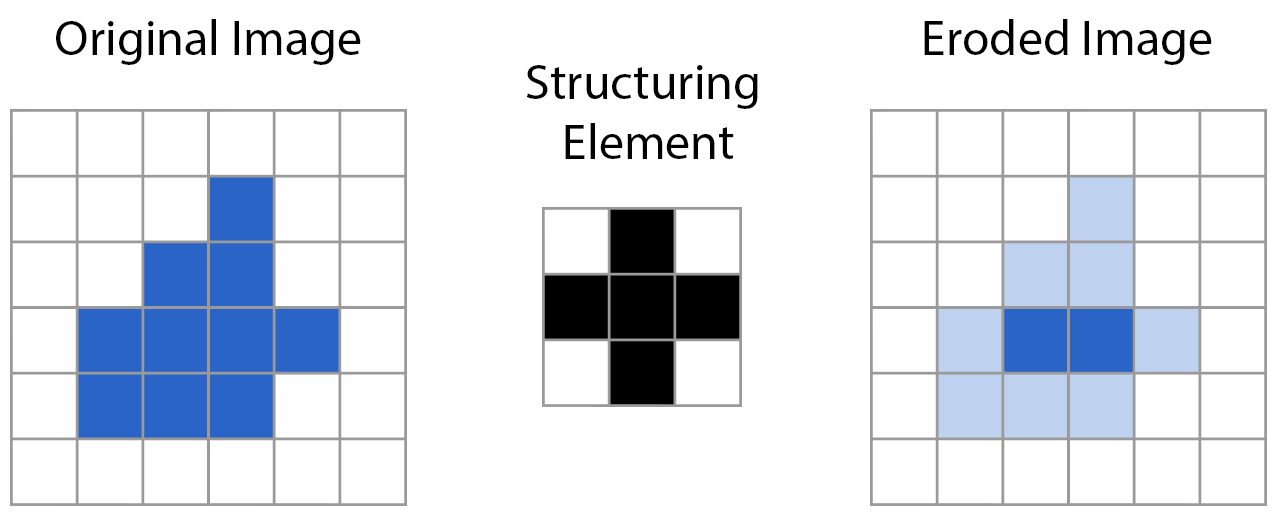
\includegraphics[scale=1]{fig/erosion.png}
  \caption{Erosion principle}
  \label{fig:erosion}
\end{figure}

\begin{figure}[h]
  \centering
  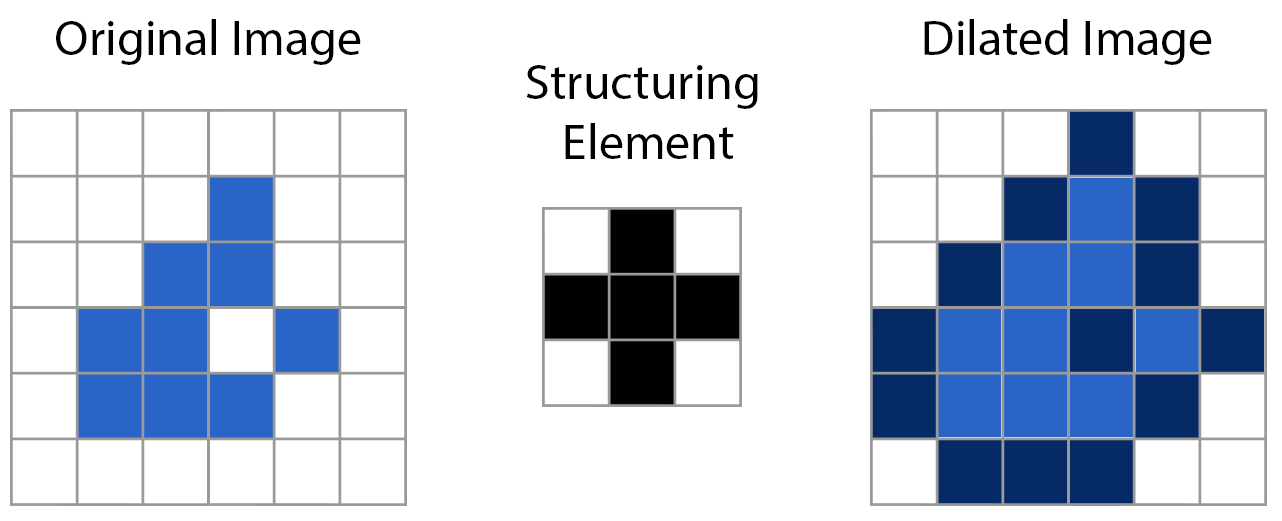
\includegraphics[scale=1]{fig/dilation.png}
  \caption{Dilation principle}
  \label{fig:dilation}
\end{figure}

\subsubsection{Erosion}
This transformation is similar to the logic gate AND. The structuring element or kernel is moved along the image and the minimal pixel value is set as the new value of the anchor point, in the figure, the center of the structuring element. This means that if all the points of the kernel are on an object (a white object on a black background), the anchor point will keep its value. On the contrary, if any element of the kernel is out of the object, the center point will become part of the background. The erosion is useful to separate two objects connected and to remove objects which are smaller than the size of the structuring element (noise). 

\subsubsection{Dilation}
The dilation is the opposite transformation of the erosion. It corresponds to the OR. If one element of the kernel is on the object (which is still assumed to have the maximal value for its pixel), the anchor point will be set to this value and thus be turned into a part of the object. This operation permits to fill holes in an object, to increase its size and to link objects which are closer than the size of the structuring element.

\subsubsection{Opening}
When combined, first by operating an erosion and then a dilation, the transformation is called an opening. The inverse operation is the closing. An opening could be convenient to separate luminous points which are connected and to then increase their size, lessen by the erosion to retrieve a shape similar to the original points.
